\subsubsection{فعالیت بالا آوردن سر}

فعالیت بالا آوردن سر یکی از فعالیت‌هایی است که می‌تواند اطلاعات مهمی درباره کنترل گردن، تنه و توانایی انجام حرکات ضدجاذبه فراهم کند. در بیماران مبتلا به ضعف عضلانی، اجرای این فعالیت ممکن است با کاهش دامنه حرکت، افزایش زمان اجرا، استفاده از الگوهای جبرانی یا ناپایداری در کنترل وضعیت سر همراه باشد. بنابراین، افزودن این فعالیت به مجموعه فعالیت‌های بررسی‌شده می‌تواند دامنه ارزیابی سامانه را کامل‌تر کند.

\paragraph{گزارش کلی فعالیت}

پس از ثبت داده‌های فعالیت بالا آوردن سر، ابتدا باید نمونه سیگنال‌های خام یا فیلترشده بررسی شوند. در این فعالیت، حسگر نصب‌شده روی پیشانی انتظار می‌رود نقش مهم‌تری نسبت به برخی فعالیت‌های دیگر داشته باشد، زیرا حرکت اصلی مربوط به تغییر وضعیت سر و گردن است. با این حال، حسگرهای دست و پا نیز می‌توانند اطلاعاتی درباره حرکات جبرانی یا تغییر وضعیت بدن فراهم کنند.

\paragraph{اهمیت ویژگی‌ها و انتخاب مؤلفه‌ها}

اثر تعداد مؤلفه‌های اصلی بر عملکرد مدل منتخب در
\autoref{fig:Sit_To_Stand_all_metrics_vs_pca}
ارائه شده است. این نمودار نشان می‌دهد که پس از حدودا ۲۰ عدد از مؤلفه‌ها، افزودن مؤلفه‌های جدید لزوماً باعث افزایش قابل‌توجه دقت نمی‌شود.

\begin{figure}[H]
	\centering
	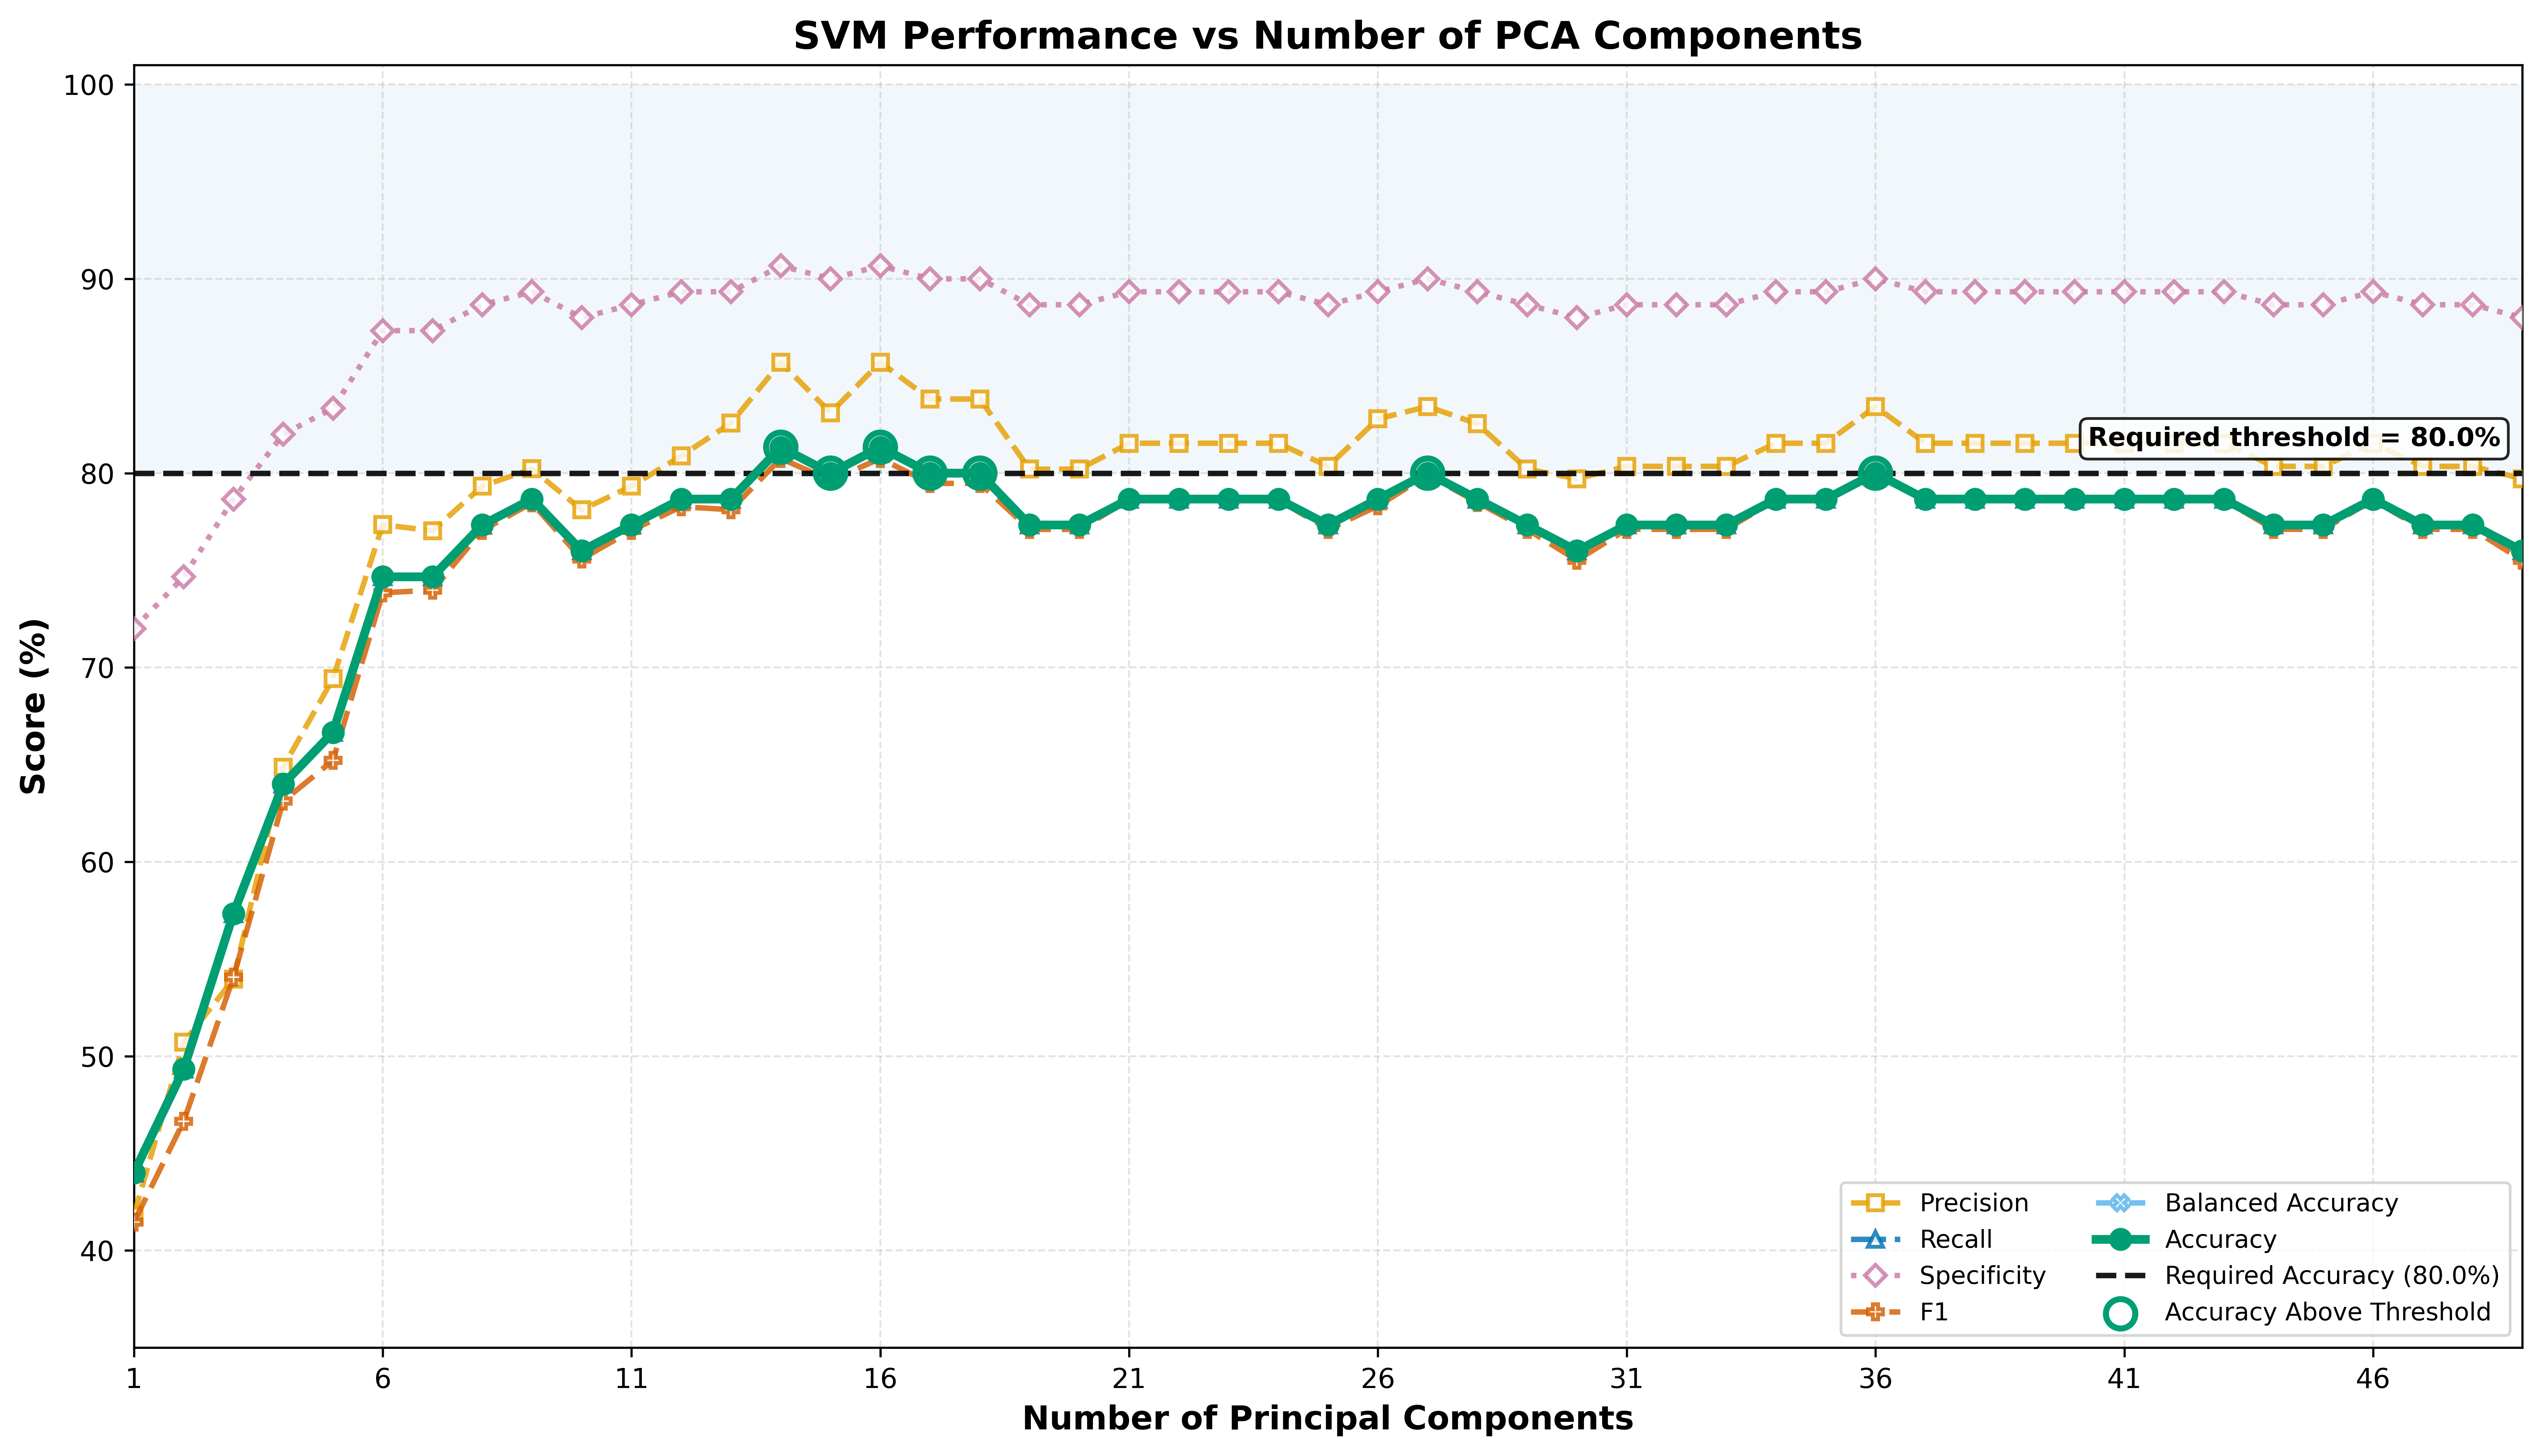
\includegraphics[width=0.8\linewidth]{../Results/Sit_To_Stand/Normal/FindPrincipalComponents_PipelinePCA_Sit_To_Stand/Figures/All_Metrics_vs_PCA}
	\caption{تغییر عملکرد مدل منتخب نسبت به تعداد مؤلفه‌های اصلی در فعالیت برخاستن از صندلی}
	\label{fig:Sit_To_Stand_all_metrics_vs_pca}
\end{figure}

در نهایت، بر اساس نمودار
\autoref{fig:Sit_To_Stand_all_metrics_vs_pca}،
مدل‌ها در بازه ۱۰ تا ۲۰ دوباره مقایسه شدند تا مدل برتر و تعداد مؤلفه‌های اصلی بهینه تعیین شود. نتیجه این مقایسه در
\autoref{fig:Sit_To_Stand_models_vs_pca_components}
ارائه شده است. بر اساس این نتایج، برای فعالیت برخاستن از صندلی مدل ماشین بردار پشتیبان با ۱۴ مؤلفه اصلی انتخاب شد. زیرا نزدیک‌ترین دقت را به معیار ۸۰ درصد داشت.

\begin{figure}[H]
	\centering
	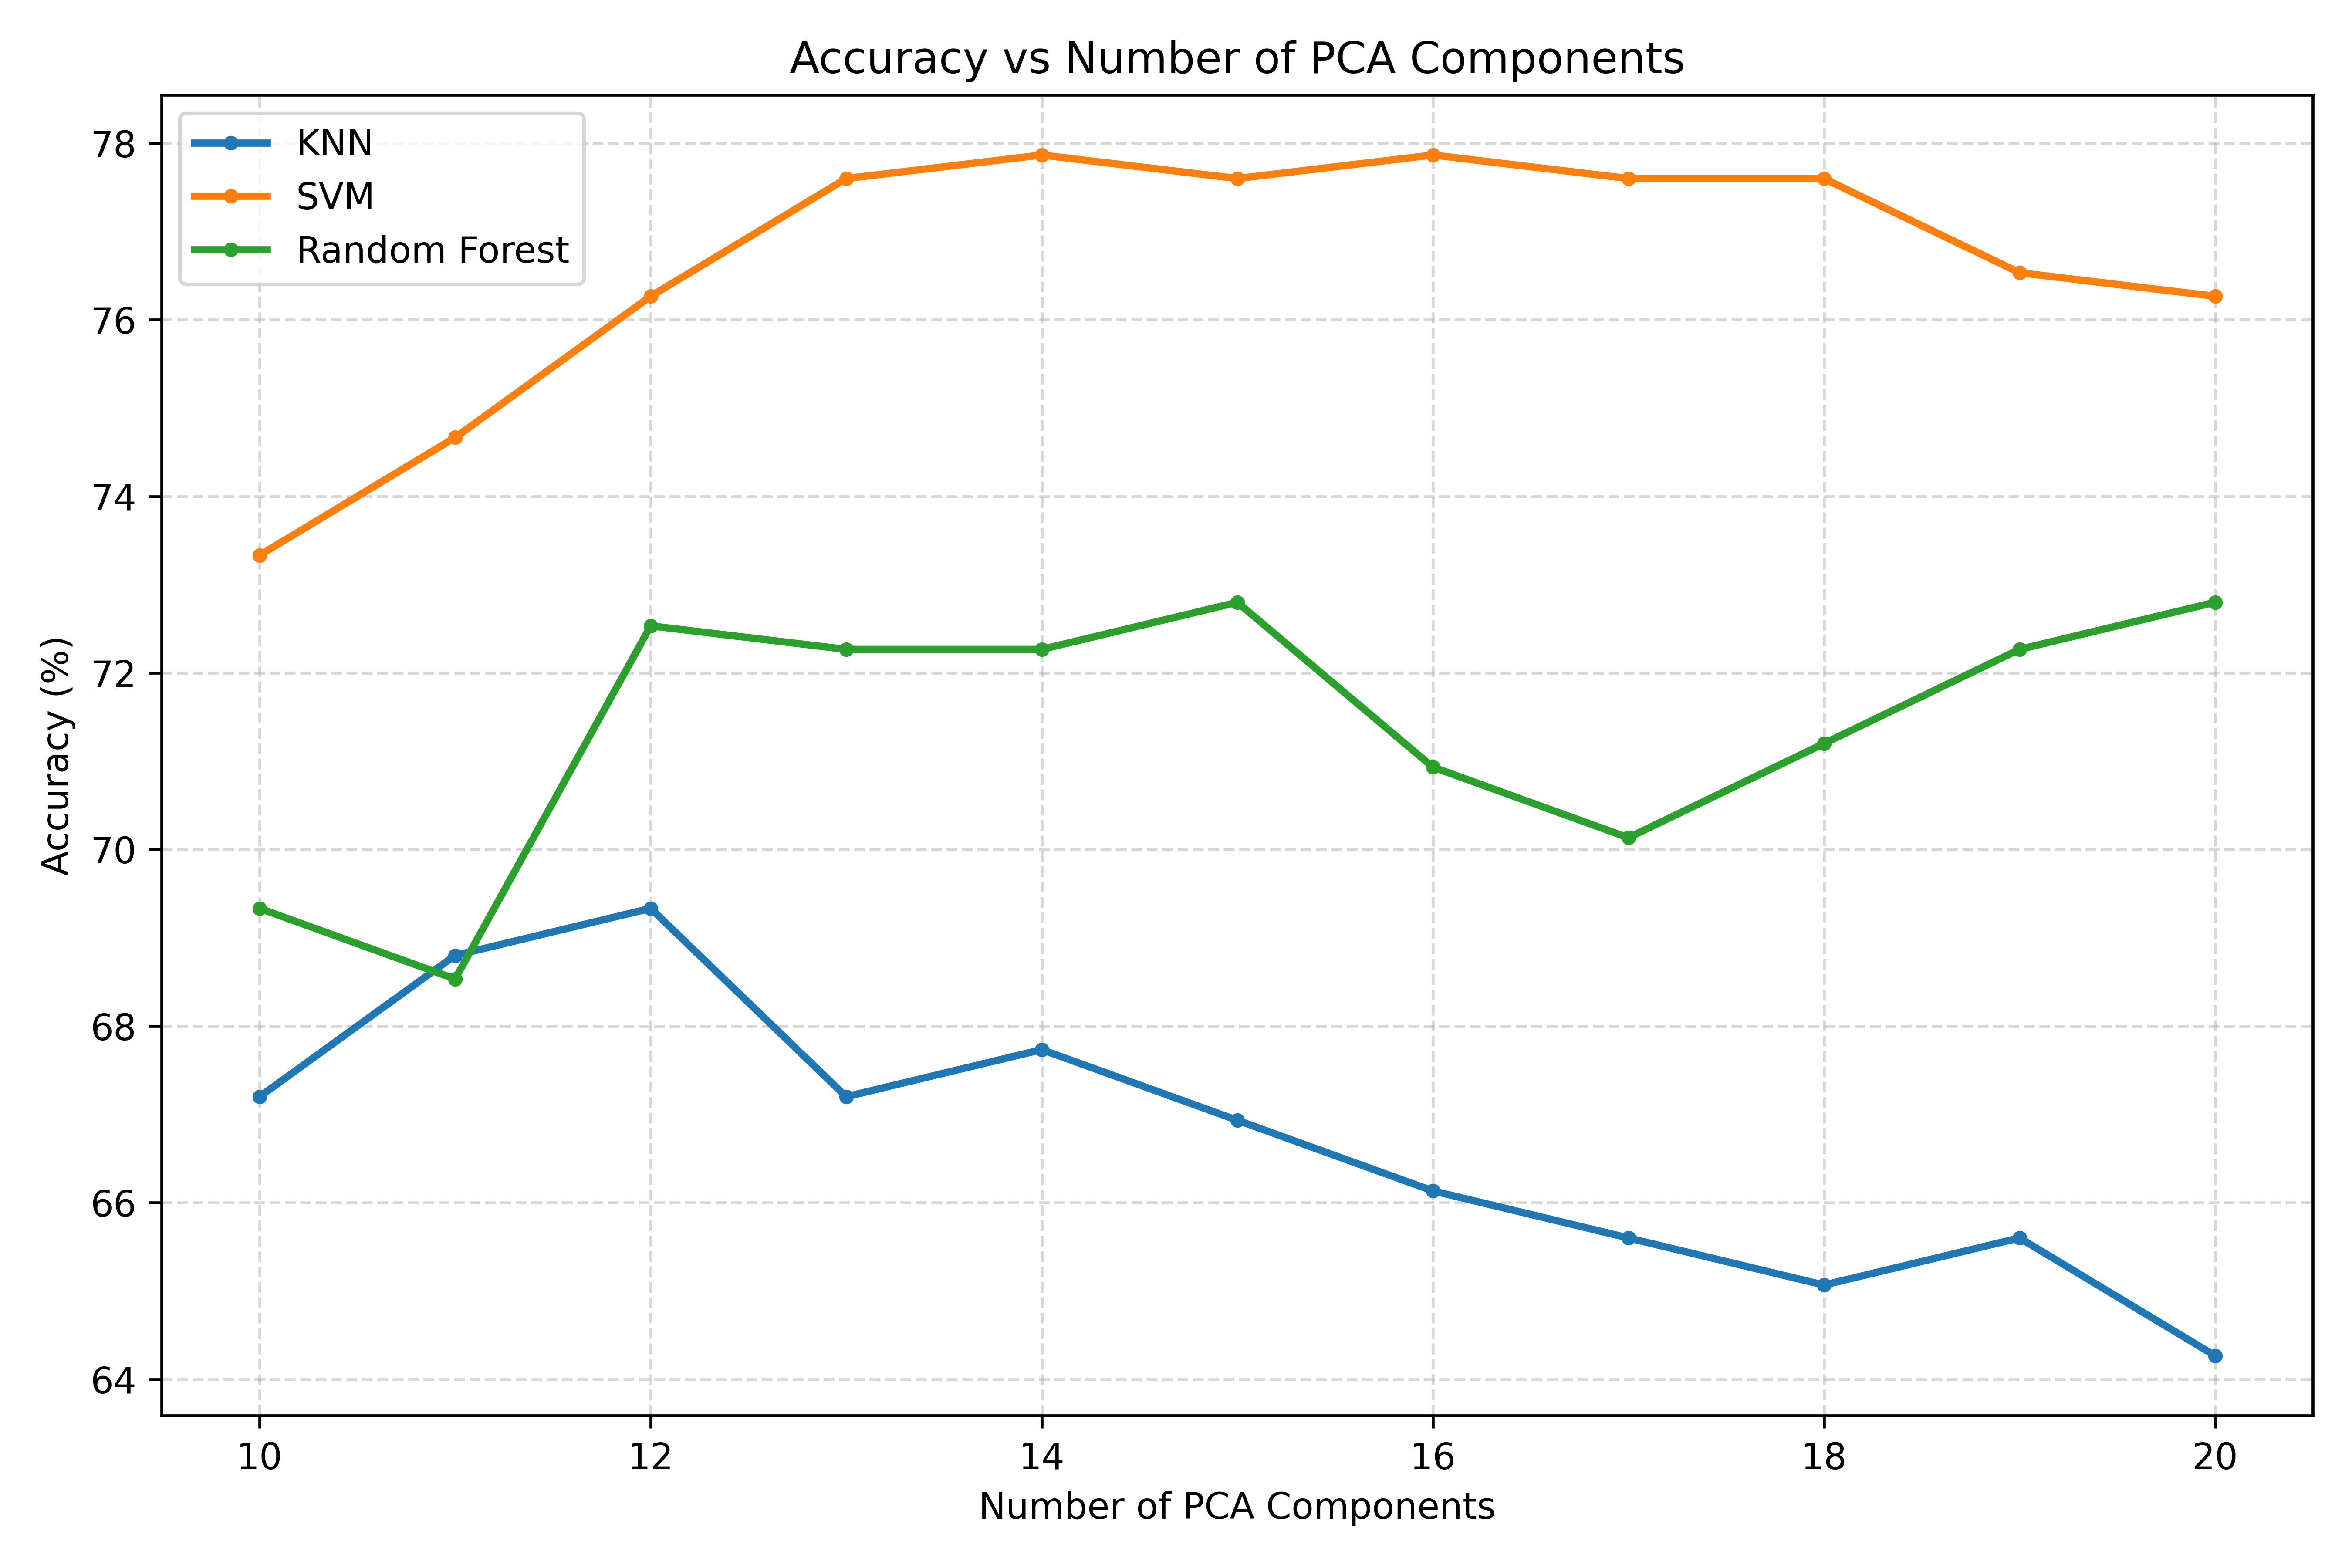
\includegraphics[width=0.8\linewidth]{../Results/Sit_To_Stand/Normal/CompareNumberOfPrincipalComponents_PipelinePCA_Sit_To_Stand/Figures/Accuracy_vs_PCA_Components}
	\caption{تغییر دقت مدل‌ها نسبت به تعداد مؤلفه‌های اصلی در فعالیت برخاستن از صندلی}
	\label{fig:Sit_To_Stand_models_vs_pca_components}
\end{figure}

\begin{table}[H]
	\centering
	\caption{تنظیمات منتخب فعالیت برخاستن از صندلی برای مدل نهایی}
	\label{tab:Sit_To_Stand_selected_setup}
	\begin{tabular}{lcccc}
		\toprule
		نوع داده & مدل منتخب & تعداد مؤلفه اصلی & معیار ارزیابی & حد نصاب معیار \\
		\midrule
		بدون جداسازی فعالیت &  ماشین بردار پشتیبان & ۱۴ & دقت & ۸۰\\
		\bottomrule
	\end{tabular}
\end{table}

\paragraph{جمع‌بندی فعالیت برخاستن از صندلی}

در فعالیت برخاستن از صندلی، مدل منتخب معرفی‌شده در
\autoref{tab:Sit_To_Stand_selected_setup}
با استفاده از اعتبارسنجی متقاطع طبقه‌بندی‌شده مورد ارزیابی قرار گرفت. نتایج نشان می‌دهند که ویژگی‌های حرکتی استخراج‌شده از حسگرها قابلیت استفاده برای تفکیک سه سطح عملکردی شبیه‌سازی‌شده این فعالیت را دارند.

توزیع واریانس مؤلفه‌های اصلی منتخب در مجموع حدود ۷۰ درصد از واریانس داده‌های اولیه را در بر می‌گیرند. این نتیجه نشان می‌دهد که برای دستیابی به عملکرد مناسب مدل، حفظ تمام واریانس داده‌ها ضروری نبوده است.

در این ارزیابی، داده‌ها در هر مرحله به ۵ بخش تقسیم شدند و فرایند اعتبارسنجی ۵ مرتبه تکرار شد. نتایج حاصل از تقسیم‌بندی‌های مختلف در
\autoref{fig:Sit_To_Stand_cv_fold_metrics}
آمده‌اند.

\begin{figure}[H]
	\centering
	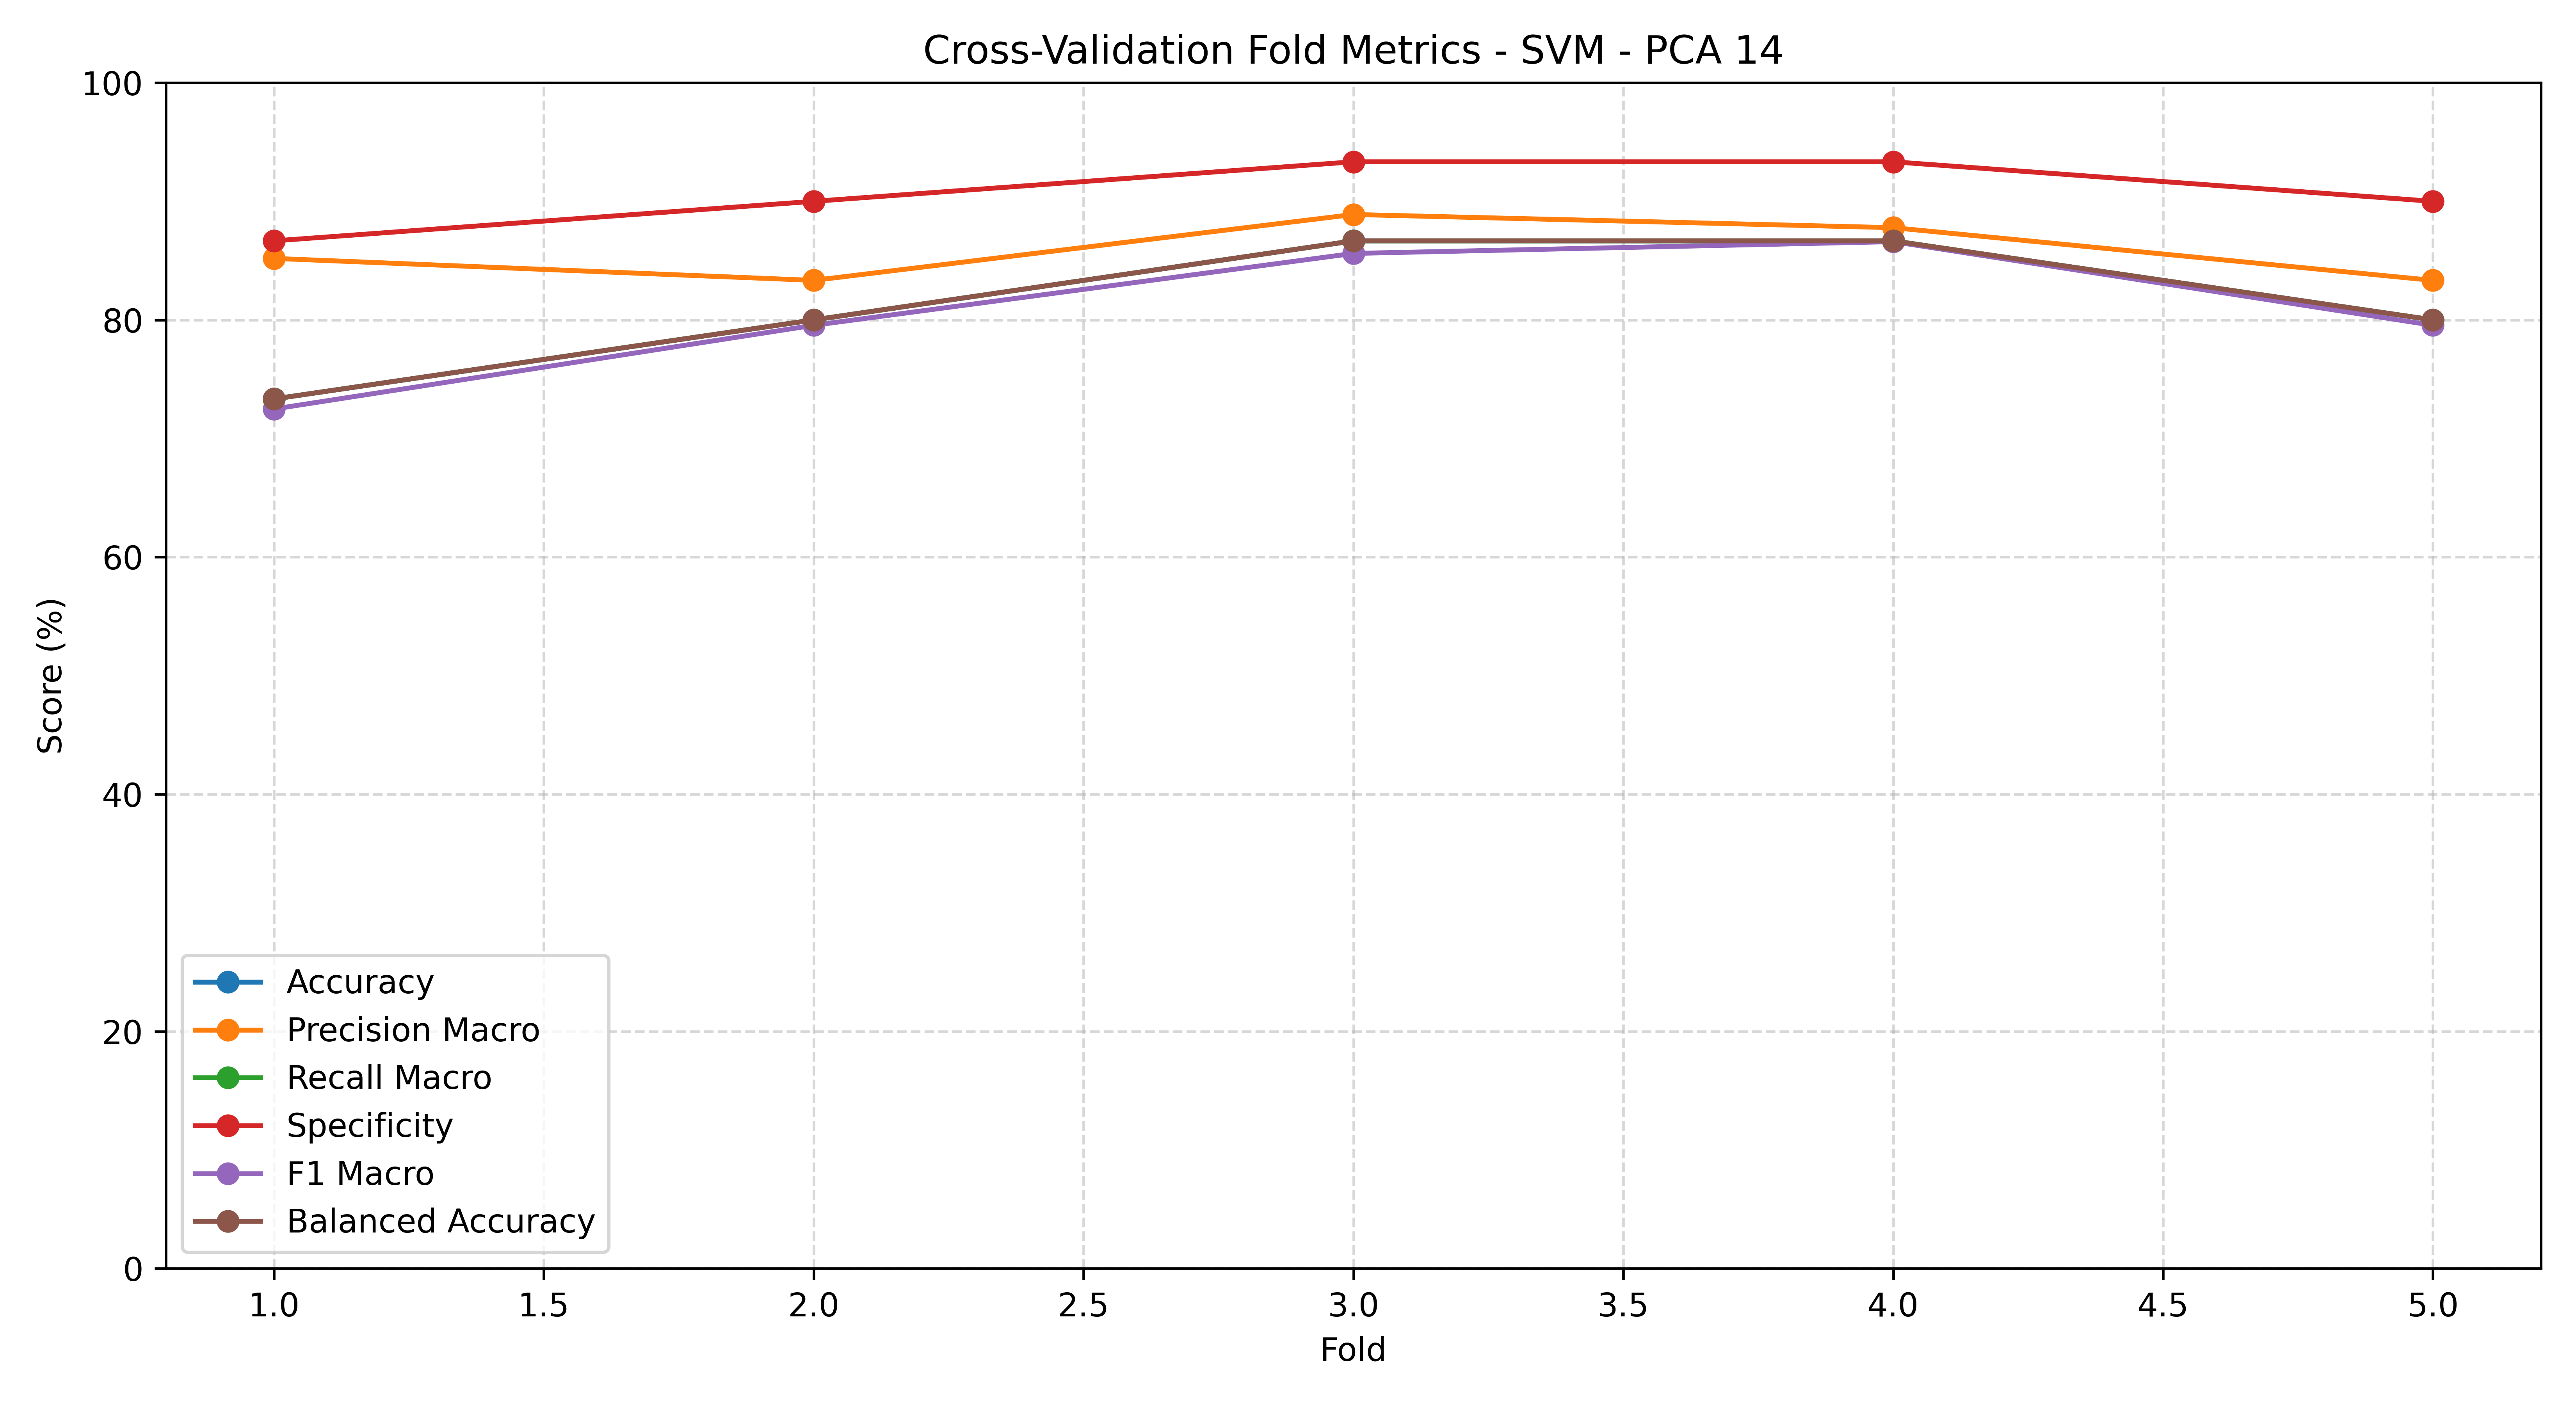
\includegraphics[width=0.8\linewidth]{../Results/Sit_To_Stand/Final/Final_Model_SVM_PCA14/Figures/CV_Fold_Metrics}
	\caption{نتایج ارزیابی مدل منتخب برای فعالیت برخاستن از صندلی در تقسیم‌بندی‌های مختلف}
	\label{fig:Sit_To_Stand_cv_fold_metrics}
\end{figure}

در مجموع، نتایج این فعالیت نشان می‌دهند که تحلیل هم‌زمان اطلاعات حسگرهای نصب‌شده روی سر، دست‌ها و پاها می‌تواند تفاوت موجود میان راهبردهای مختلف برخاستن از روی صندلی را آشکار کند. 
